\hyt{morseovka}
\song{Morseovka}

\note{capo 4}

\vers{1}{
\chord{D}Pámbu \chord{E\7}mi dal \chord{A}dárek, \chord{G}tu nejhezčí \chord{A}z Klá\chord{D}rek.\\
\chord{G}Kvůli jejím očím \chord{Hm}kočár s panem kočím \chord{G}předěláme \chord{A}na ko\chord{D}čárek.
}

\solon{1}{
	
\vspace{-30pt}
\hspace{21pt}
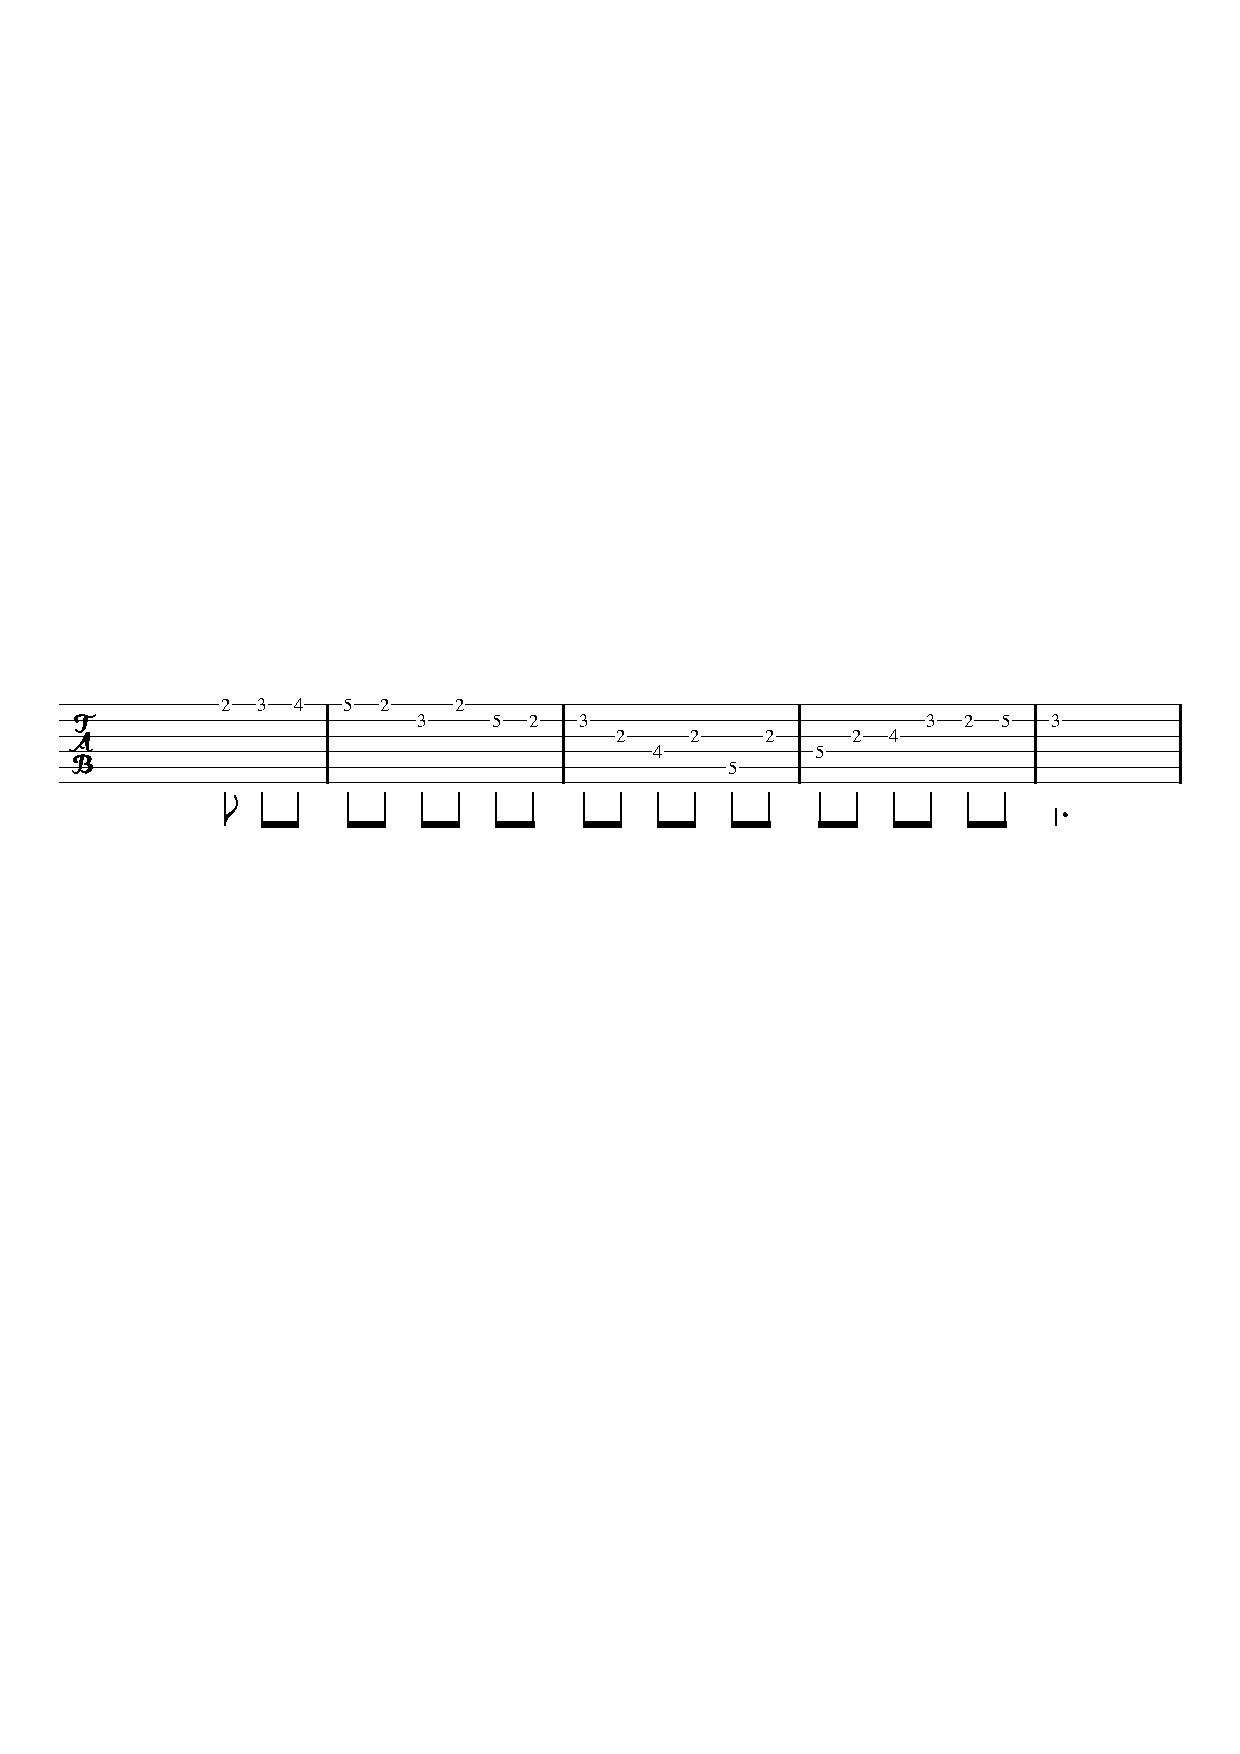
\includegraphics[width=\linewidth]{scores/morseovkasolo1.pdf}
}
\vspace{-30pt}

\refrainn{1}{
\chord{Hm}Na nebi se \chord{F\kk m}pasou \chord{Hm}ovce, co znamená \chord{A}v morse\chord{D}ovce \chord{G}čárka, tečka, \chord{F\kk m}čárka?\\
\chord{G}Tak začíná, \chord{G\bas{F\kk}}tak začíná, \chord{G\bas{E}}tak začíná \chord{A}Klár\chord{D}ka.
}

\solon{2}{
	
\vspace{-30pt}
\hspace{21pt}
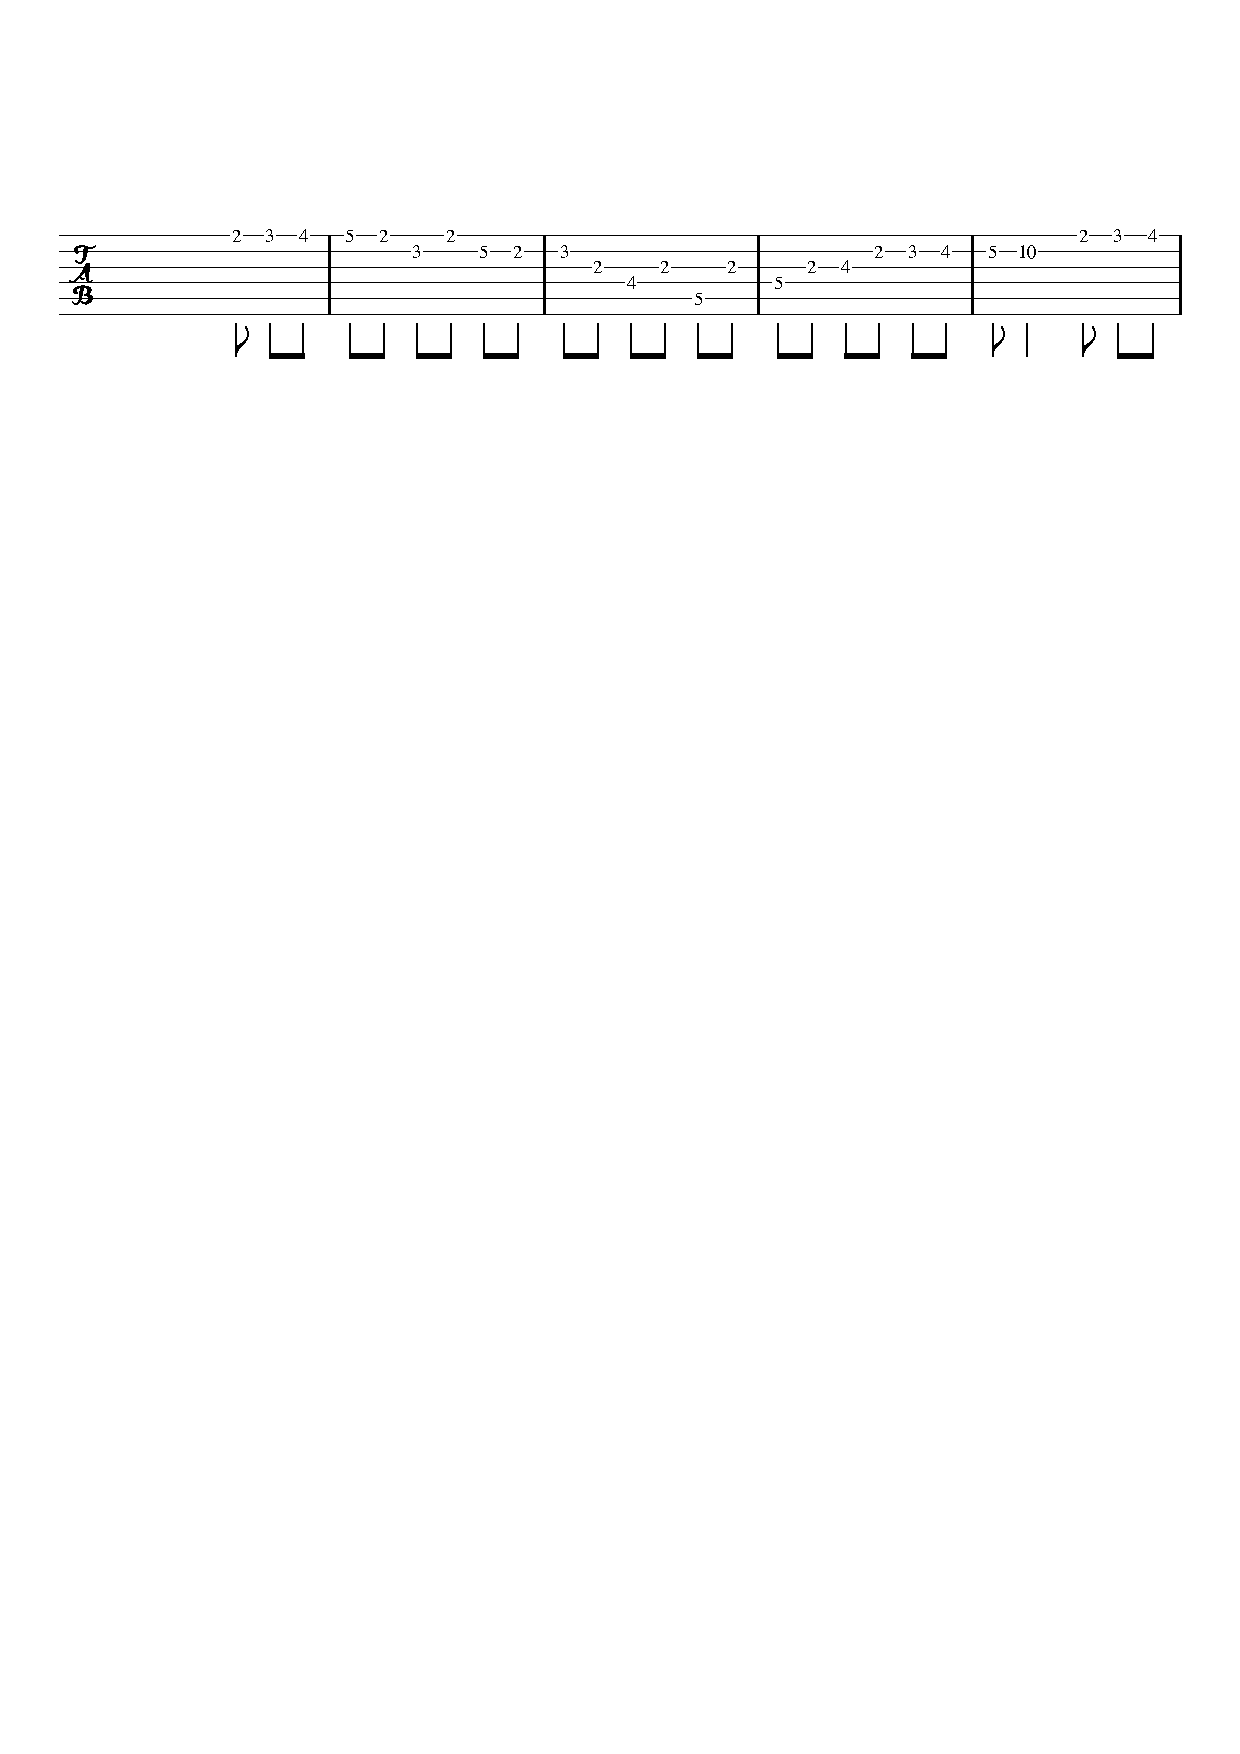
\includegraphics[width=\linewidth]{scores/morseovkasolo2.pdf}

\vspace{-7pt}
\hspace{20.5pt}
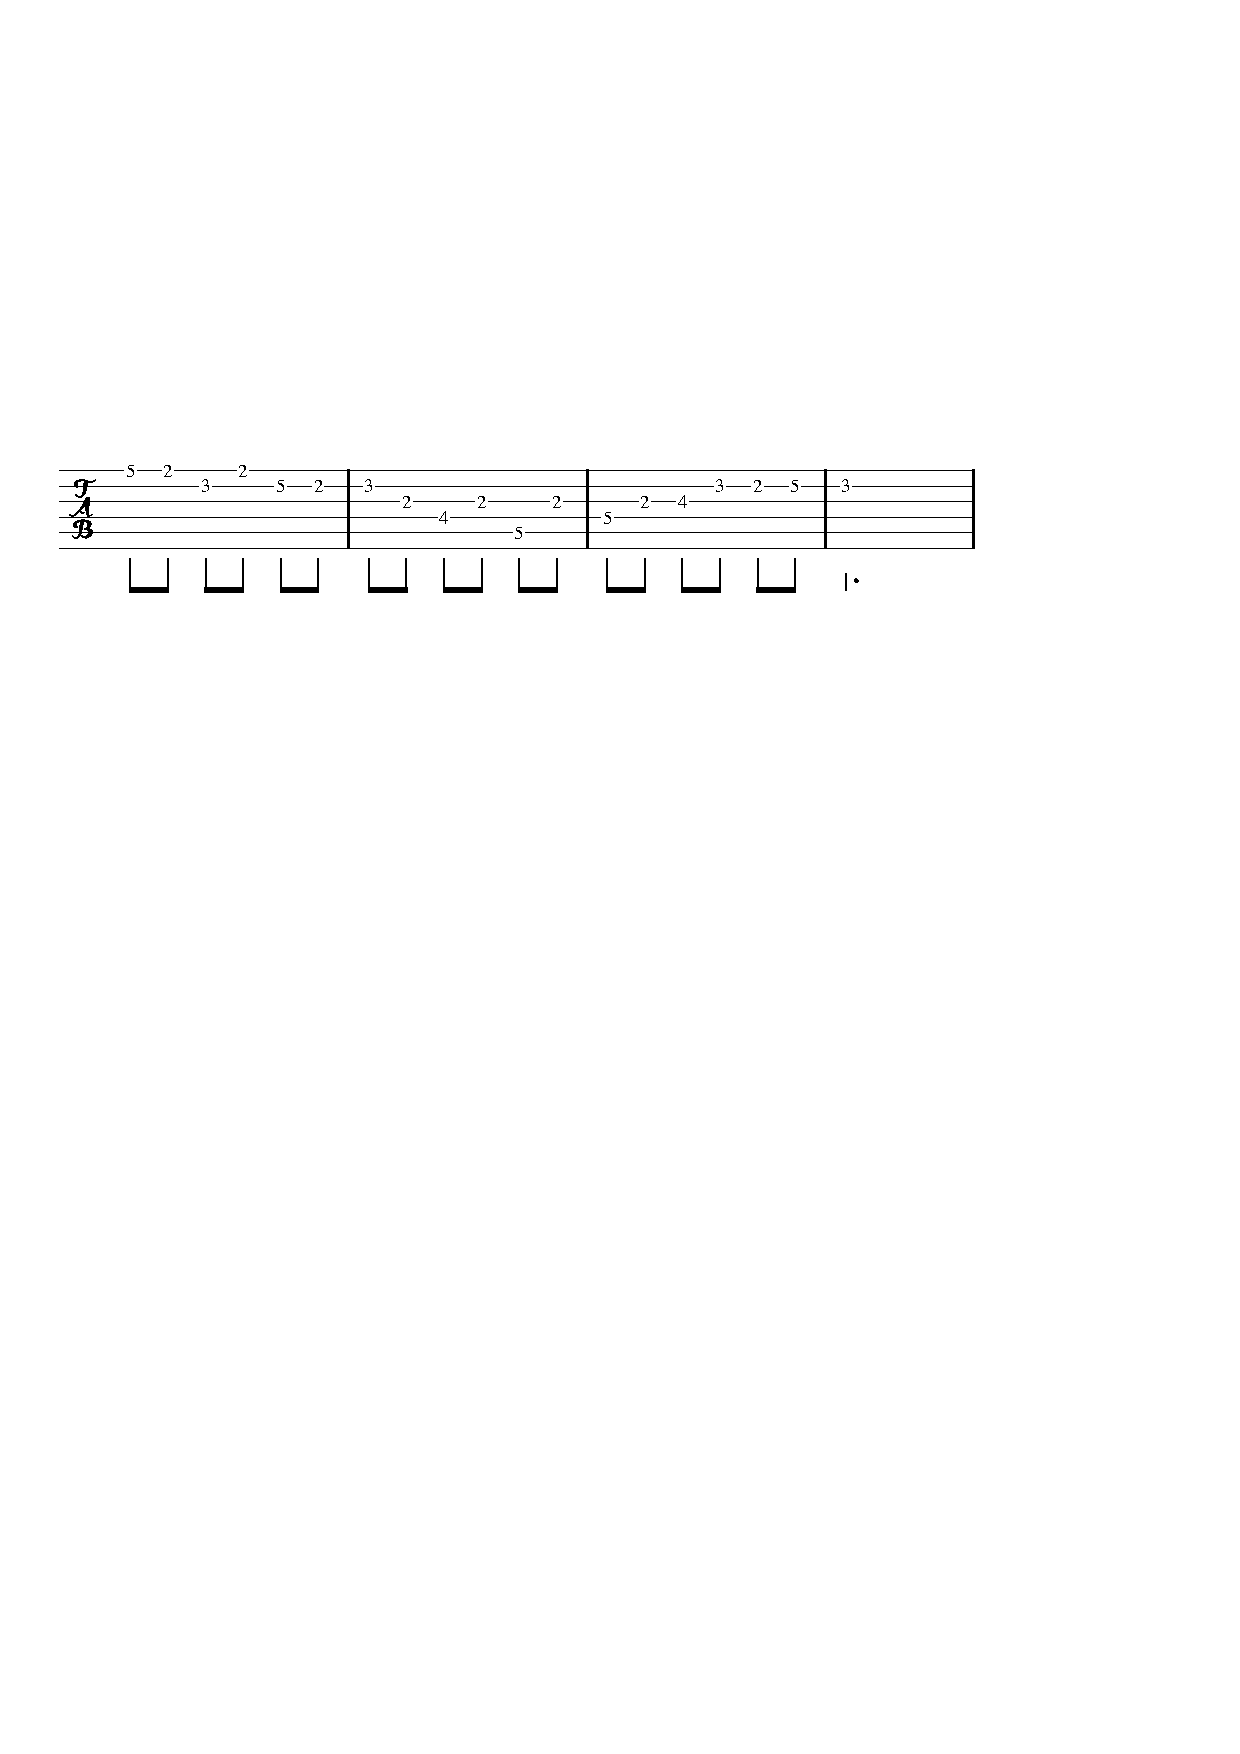
\includegraphics[width=\linewidth]{scores/morseovkasolo3.pdf}
}
\vspace{-20pt}

\vers{2}{
Pámbu dělá zmatky, náruč paní Katky\\
způsobila to, že volám, Pane Bože, vem si svoji Kláru zpátky.
}

\solosm{1}

\refrainn{2}{
Noční šelma volá lovce, co znamená v morseovce čárka, tečka, čárka?\\
Tak začíná, tak začíná, tak začíná Katka.
}

\solosm{2}

\vers{3}{
Co mi zbejvá k stáru? Noční můry v denním báru.\\
Duševně jsem chorým pro lásku a pro rým, Pane Bože, vrať mi Kláru.
}

\solosm{1}

\refsm{1}
\ns

\solosm{2}
\newpage
